%%%%%%%%%%%%%%%%%%%%%%%%%%%%%%%%%%%%%%%%%
% Beamer Presentation
% LaTeX Template
% Version 1.0 (10/11/12)
%
% This template has been downloaded from:
% http://www.LaTeXTemplates.com
%
% License:
% CC BY-NC-SA 3.0 (http://creativecommons.org/licenses/by-nc-sa/3.0/)
%
%%%%%%%%%%%%%%%%%%%%%%%%%%%%%%%%%%%%%%%%%

%----------------------------------------------------------------------------------------
%	PACKAGES AND THEMES
%----------------------------------------------------------------------------------------

\documentclass{beamer}

\mode<presentation> {

% The Beamer class comes with a number of default slide themes
% which change the colors and layouts of slides. Below this is a list
% of all the themes, uncomment each in turn to see what they look like.

%\usetheme{default}
%\usetheme{AnnArbor}
%\usetheme{Antibes}
%\usetheme{Bergen}
%\usetheme{Berkeley}
%\usetheme{Berlin}
%\usetheme{Boadilla}
%\usetheme{CambridgeUS}
%\usetheme{Copenhagen}
%\usetheme{Darmstadt}
%\usetheme{Dresden}
%\usetheme{Frankfurt}
%\usetheme{Goettingen}
%\usetheme{Hannover}
%\usetheme{Ilmenau}
%\usetheme{JuanLesPins}
%\usetheme{Luebeck}
\usetheme{Madrid}
%\usetheme{Malmoe}
%\usetheme{Marburg}
%\usetheme{Montpellier}
%\usetheme{PaloAlto}
%\usetheme{Pittsburgh}
%\usetheme{Rochester}
%\usetheme{Singapore}
%\usetheme{Szeged}
%\usetheme{Warsaw}

% As well as themes, the Beamer class has a number of color themes
% for any slide theme. Uncomment each of these in turn to see how it
% changes the colors of your current slide theme.

%\usecolortheme{albatross}
%\usecolortheme{beaver}
%\usecolortheme{beetle}
%\usecolortheme{crane}
%\usecolortheme{dolphin}
%\usecolortheme{dove}
%\usecolortheme{fly}
%\usecolortheme{lily}
%\usecolortheme{orchid}
%\usecolortheme{rose}
%\usecolortheme{seagull}
%\usecolortheme{seahorse}
%\usecolortheme{whale}
%\usecolortheme{wolverine}

%\setbeamertemplate{footline} % To remove the footer line in all slides uncomment this line
%\setbeamertemplate{footline}[page number] % To replace the footer line in all slides with a simple slide count uncomment this line

%\setbeamertemplate{navigation symbols}{} % To remove the navigation symbols from the bottom of all slides uncomment this line
}
\usepackage{amsmath}
\usepackage{multirow}
\usepackage{caption}% http://ctan.org/pkg/caption
\usepackage{graphicx} % Allows including images
\usepackage{booktabs} % Allows the use of \toprule, \midrule and \bottomrule in tables
\captionsetup[figure]{labelformat=empty}%
%----------------------------------------------------------------------------------------
%	TITLE PAGE
%----------------------------------------------------------------------------------------

\title[Autononous Parking Space Detection]{Autonomous Parking Space Detection} % The short title appears at the bottom of every slide, the full title is only on the title page

\author[Julien Nyambal 1439552]{Julien Nyambal\\1439552} % Your name
\institute[WITS] % Your institution as it will appear on the bottom of every slide, may be shorthand to save space
{
School of Computer Science and Applied Mathematics\\ % Your institution for the title page
University of the Witwatersrand, Johannesburg \\
\medskip
%\textit{john@smith.com} % Your email address
Supervisor: Dr. Richard Klein \\
\medskip
\large Master's Proposal
\vspace{0.3cm}

\begin{figure}
	
\includegraphics[width=0.1\linewidth]{Pictures/wits1}
	\label{fig:wits1}
\end{figure}


}




\date[\today]{} % Date, can be changed to a custom date

\begin{document}

\begin{frame}
\titlepage % Print the title page as the first slide
\end{frame}

\begin{frame}
\frametitle{Overview} % Table of contents slide, comment this block out to remove it
\tableofcontents % Throughout your presentation, if you choose to use \section{} and \subsection{} commands, these will automatically be printed on this slide as an overview of your presentation
\end{frame}

%----------------------------------------------------------------------------------------
%	PRESENTATION SLIDES
%----------------------------------------------------------------------------------------

%------------------------------------------------
\section{Introduction} % Sections can be created in order to organize your presentation into discrete blocks, all sections and subsections are automatically printed in the table of contents as an overview of the talk
%------------------------------------------------

\begin{frame}
\Huge Introduction
\end{frame}

\subsection{Description}

\begin{frame}
\frametitle{Description}

The project aims to automatically predict the availability of a parking spot given the feeds provided by a video camera monitoring the parking area. 

\end{frame}

%--------------------------------------------------------
\subsection{Motivation}

\begin{frame}
\frametitle{Motivation}

\begin{block}{\textbf{Hunting for parking brings no joy for students}\cite{wits}}
``...Students at Wits are struggling to find available parking spaces on campuses since...''\\ 
``...student X said that finding parking is the biggest issue she faces at Wits.''
\\[5pt]
\rightline{{\rm --- Aarti Bhana, Wits Vuvuzela}}
\end{block}
\end{frame}

%------------------------------------------------
\subsection{Problems}
\begin{frame}
\frametitle{Problems}
Various factors can explain the parking space problems mostly in urban areas:

\begin{itemize}
\item Urban planning not following the quick growth of population dynamics
\item Drivers not aware of available space due to lack of knowledge of the area or anything obstructing it from the driver 
\item Bad management of the parking area
\end{itemize}
\end{frame}

%------------------------------------------------
\subsection{Aims}
\begin{frame}
\frametitle{Aims}

This project aims to:

\begin{itemize}
\item Perform comparative study between existing solutions (SVM based algorithms) and CNN,
\item Use video cameras to allocate parking spaces to drivers
\item Apply computer vision techniques to infer the status of a space (Background subtraction, Hough transform ...),
\item Help the driver to locate a vacant spot using the dedicated web application,
\item Run a quantitative analysis of the results produced by the system to predict parking habits of drivers.
\end{itemize}

\end{frame}

%------------------------------------------------
\section{Background and related work}
%------------------------------------------------

\begin{frame}
\Huge Background and related work
\end{frame}

\subsection{Sensors Based Detection}

\begin{frame}
\frametitle{Sensors Based Detection}

\begin{figure}[!htbp]
  \centering
  \begin{minipage}[b]{0.5\textwidth}
    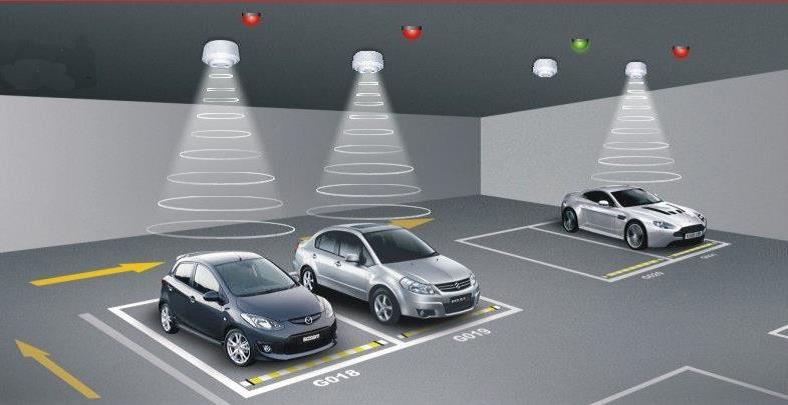
\includegraphics[width=\textwidth]{Pictures/overhead}
    \caption{Non-intrusive sensors, \cite{overhead}}
    \label{nonintru}
  \end{minipage}
  \hfill
  \begin{minipage}[b]{0.4\textwidth}
    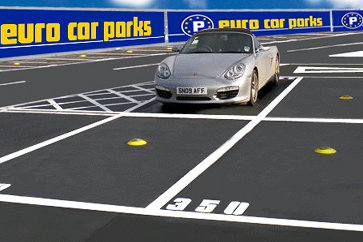
\includegraphics[width=\textwidth]{Pictures/sensor}
    \caption{Intrusive sensors, \cite{ground}}
    \label{intru}
  \end{minipage}
\end{figure}

\end{frame}

\begin{frame}
\frametitle{Sensors Based Detection}

Pros:
\begin{itemize}
	\item Very accurate,
	\item Since individually installed per spot, the system can return the available number of spots \cite{Lee2008},
	\item Almost no computation required
\end{itemize}

Cons:
\begin{itemize}
	\item Expensive in installation in terms of number of devices to place per spot,
	\item Expensive in maintenance.
\end{itemize}

\end{frame}
%------------------------------------------------

\subsection{Video Based Methods}

\begin{frame}[allowframebreaks]
\frametitle{Background Subtraction}
\begin{block}{Definition}
The background subtraction is a technique used in computer vision and image processing for detecting the foreground from a set a images of the same scenario (video sequence of a non-moving camera) for various types of detection problems.

\[
pixel\_value= 
\begin{cases}
1,& |frame_i - frame_{i-1}| > T_h\\
0,              & \text{otherwise}
\end{cases}
\]
%\begin{equation}
%|frame_i - frame_{i-1}| > T_h 
%\label{diff_frame}
%\end{equation}
\end{block}
\vspace{5cm}
\begin{figure}[!htbp]
	\begin{minipage}[b]{0.48\textwidth}
		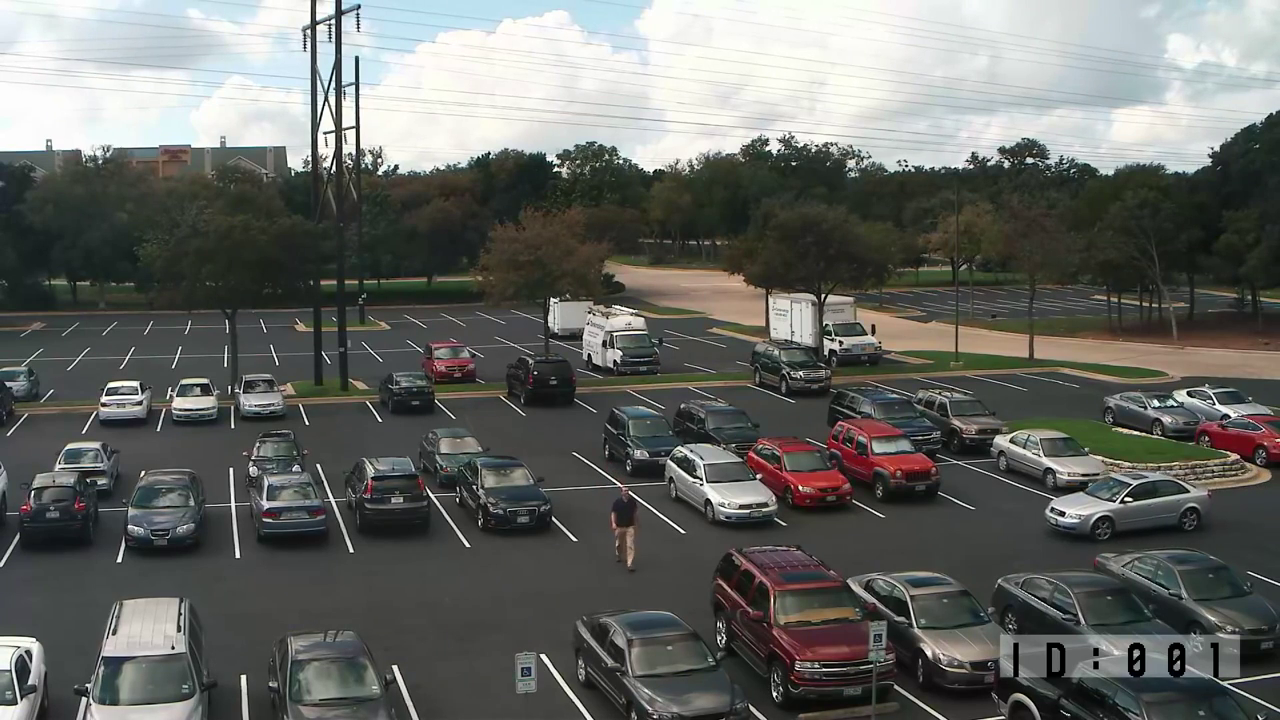
\includegraphics[width=\textwidth]{Pictures/fg308}
		\caption{Original image}
		\label{foreground}
	\end{minipage}
	\hfill
	\begin{minipage}[b]{0.48\textwidth}
		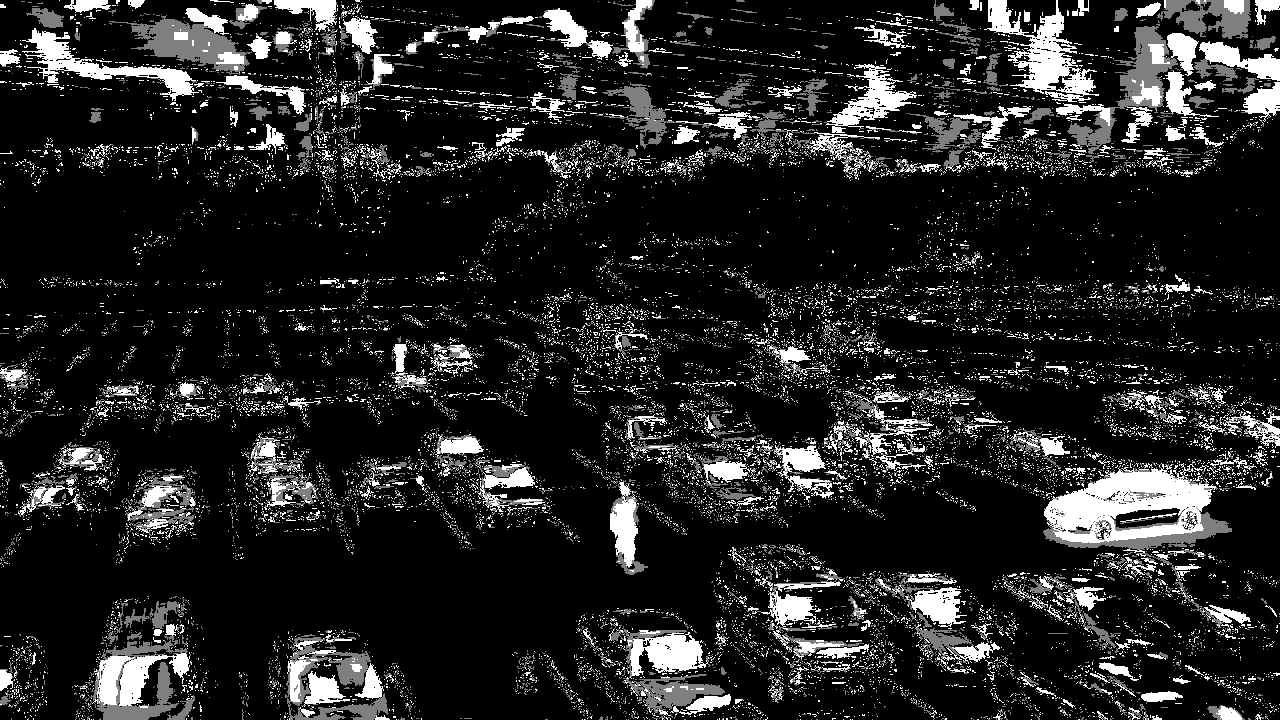
\includegraphics[width=\textwidth]{Pictures/bg308}
		\caption{Background subtracted image}
		\label{background}
	\end{minipage}
\end{figure}
\vspace{5cm}
Background subtraction to:
\begin{itemize}
	\item Create a transience map of the parking area or to model the parking area given the previous positions of vehicles \cite{Postigo}
	\begin{figure}
		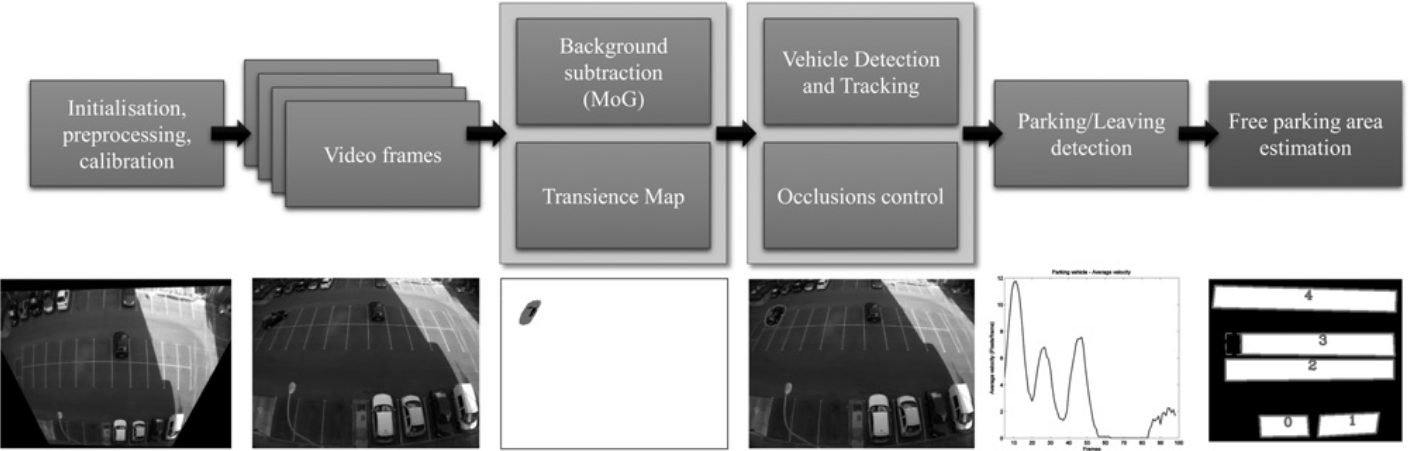
\includegraphics[width=300pt]{Pictures/transmap}
		\caption{Background subtraction method proposed by \cite{Postigo}}
		\label{postigo}
	\end{figure}
	This method used the background subtraction and the Mixture of Gaussians to detect and track vehicles to infer the availability of remaining spots given a \textbf{threshold} on the transient value, 
	\item Use histograms of spatial features to map the spots of an unmanaged parking area but taking as object the group of pixels generated by vehicles, rejecting the non-vehicle objects by automatically adjusting the \textbf{threshold} \cite{Choeychuen}.
\end{itemize}


\end{frame}

\begin{frame}[allowframebreaks]
\frametitle{Support Vector Machines}
\textbf{Definition:}\\
Supervised machine learning technique that is based on a decision boundary to separate data into different subsets (classes). Support vectors are the coordinates of data point in the data space that are the closest to the boundary lines, hyperplanes.\\
Support Vector Machines(SVM) can be used for \textbf{classification} and \textbf{regression} problems. The classification has been mostly used for the parking space detection.

\begin{figure}[h!]
	%should be after intrinsic calibration
	\centering
	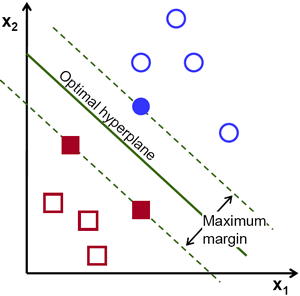
\includegraphics[width=0.3\textwidth]{Pictures/SVM}
	\caption{Support Vector Machines, OpenCVDocs}
\end{figure}

Support Vector Machines (SVM) have been widely used for the problem. Usually associated with Histograms of Oriented Gradients (HoG), Difference of Gaussians (DoG), color histograms, Local Binary Patterns...

\begin{itemize}
	\item To detect available parking spaces using both multi-class Support Vector Machines (SVMs) and a Markov Random Field (MRF) framework using the color histograms as features \cite{wu} with an accuracy of 93.52\%,
	\begin{figure}[h!]
		%should be after intrinsic calibration
		\centering
		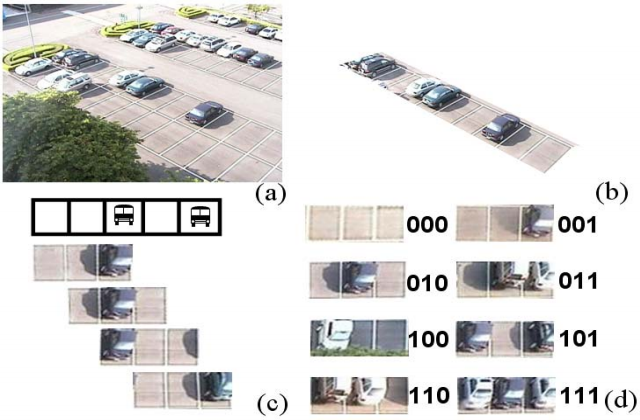
\includegraphics[width=0.4\textwidth]{Pictures/Wu}
		\caption{Multi-class SVM, \cite{wu}}
	\end{figure}
	\item To classify individual spot using DoG- features with an accuracy of 92.33 after a comparative study with the k-NN, LDA and HoG, RGB, HSV YUV (color spaces) as features \cite{Tschentscher}\%
	\item As similar to the previous point,to classify individual spot using Local Binary Patterns and Local Phase Quantization as features with an accuracy of 99\% \cite{deAlmeida}.
	
		\begin{figure}[h!]
		%should be after intrinsic calibration
		\centering
		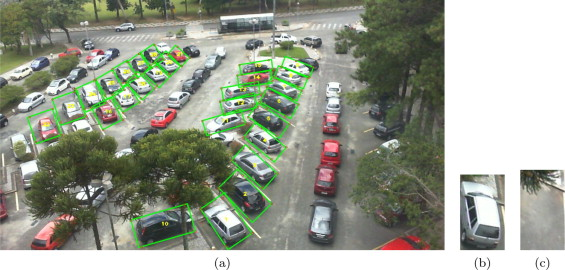
\includegraphics[width=0.8\textwidth]{Pictures/parking}
		\caption{Segmented image, \cite{deAlmeida}}
	\end{figure}
	
\end{itemize}

\end{frame}

\begin{frame}[allowframebreaks]
\frametitle{Deep Learning - Convolutional Neural Networks }

\begin{block}{Definition}

\begin{itemize}
\item Supervised learning branch of machine learning for pattern and object recognition,
\item CNN learn extracted features,
\item CNN are computationally expensive at the training phase especially when the dataset contains many classes with many objects to classify,
\item But high accuracy compared to its direct competitor the SVMs.
\end{itemize}

\end{block}

\begin{figure}[h!]
%should be after intrinsic calibration
    \centering
    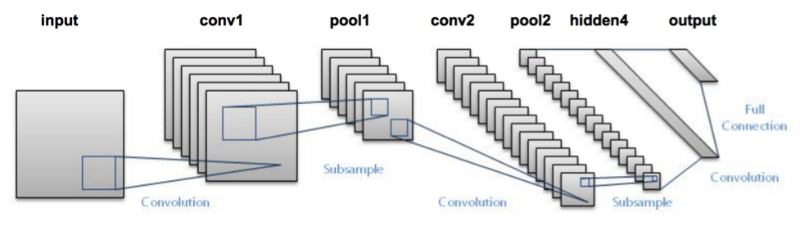
\includegraphics[width=0.9\textwidth]{Pictures/lenet_architecture}
    \caption{Overview of a CNN: Lenet-5, \cite{Lecun98gradient-basedlearning}}
\end{figure}

\begin{figure}[h!]
	%should be after intrinsic calibration
	\centering
	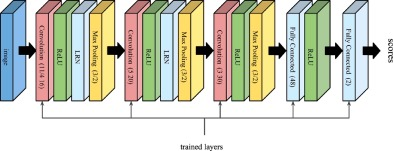
\includegraphics[width=0.9\textwidth]{Pictures/deep}
	\caption{Modern CNN, mini-AlexNet, \cite{NIPS2012_4824,Amato2017327}}
\end{figure}

\framebreak

CNNs to bring a solution to parking management:

\begin{itemize}
	\item The classification happens in a remote server that is fed with images coming from cameras facing a parking area. 
	\begin{figure}[h!]
		%should be after intrinsic calibration
		\centering
		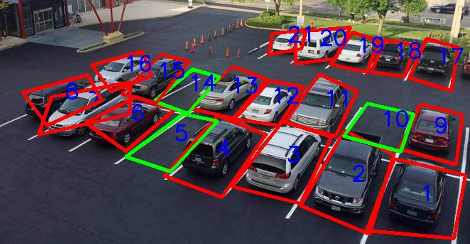
\includegraphics[width=0.8\textwidth]{Pictures/stall}
		\caption{Online classification, \cite{7845408}}
	\end{figure} 
	\item The classification happens in individual customized cameras that contain Raspberry Pi's. Each camera runs a reduced version of AlexNet CNN \cite{Amato2017327}. 
\end{itemize}


\end{frame}

%----------------------------------------
\section{Research Methodology}

\begin{frame}
\Huge Research Methodology
\end{frame}

\subsection{Research Hypothesis}

\begin{frame}
\frametitle{Research Hypothesis}
\begin{itemize}
	\item \textbf{Hypothesis1: }Hough Transform for lines detection which implies spot presence (on the first frame) + CNN for classification,
	\item \textbf{Hypothesis2: }Hough Transform for lines detection + Background Subtraction to the incoming frame from the camera to automatically segment the image for parking spaces through their lines + SVM * (Histograms of Oriented Gradients OR  Difference of Gaussians OR Local Binary Patterns ...),
	\item \textbf{Hypothesis3: } RCNN for spots detection + (SVM OR Normal-CNN) OR (trained-Normal-CNN AND CNN-learned-features-SVM) for spots classification.
\end{itemize}

\end{frame}

\subsection{Research Questions}

\begin{frame}
\frametitle{Research Questions}
\begin{itemize}
	\item Do the background subtraction and the Hough transform associated with the Convolutional Neural Networks and the Support Vector Machines efficiently return automatically the status of all the parking spaces?
	\item Will the RCNN be better at automatically detect the spots without human intervention?
	\item How could the union of the features generated by a trained CNN and the power of the SVM improve the classification accuracy and credibility of the parking space management? 
\end{itemize}
\end{frame}

\subsection{Methodology}

\begin{frame}
\frametitle{Background Subtraction}
\textbf{Method 1:} 
\begin{itemize}
	\item To automatically create a mapping of all the parking spaces given a parking lot as illustrated in Section \ref{postigo} when using the transience map \cite{Postigo},
	\item From the map, feed the cropped spot to either the CNNs or SVMs.
\end{itemize}

\textbf{Method 2:}
\begin{itemize}
	\item To use GrabCut on one image of the parking space to crop the background from the foreground, create a map (ground-truth) out of GrabCut
	\item And classify the results using CNNs or SVMs. 
\end{itemize}  
\end{frame}

\begin{frame}
\frametitle{Hough Transform}
Parking spots contain lines that can be detected using the Hough Transform. The end-points of those lines will joint altogether by the Convex Hull algorithm to create rectangle of spots to build a map (ground-truth) of the parking area and classify each spot per frame.
\begin{figure}
	\centering
	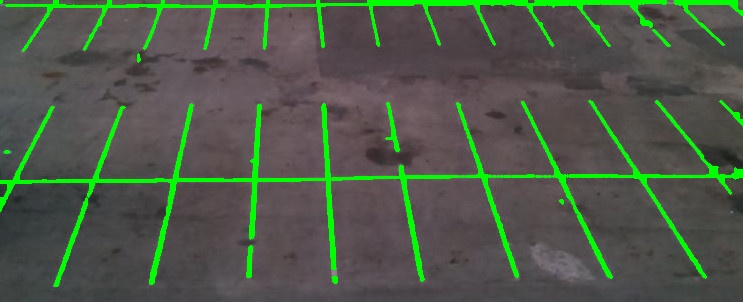
\includegraphics[width=0.7\linewidth]{Pictures/output_houghl}
	\caption{Result of Hough Transform}
	\label{fig:outputhoughl}
\end{figure}
\end{frame}

\begin{frame}
\frametitle{Convolutional Neural Networks: CNN}
\begin{itemize}
	\item \textbf{Method 1:} To reduce the depth of the successfull AlexNet, since 2 classes in the project, instead of 1000,
	\item \textbf{Method 2:} A new CNN will be created using state-of-the-art rules for CNN design. CNN design is an art that follows some rules to have both speed and specially accuracy.  
\end{itemize}
\end{frame}

\begin{frame}
\frametitle{Region-based Convolutional Neural Networks: R-CNN}

The algorithm will be ran on one frame of the parking area of interest to return the coordinates of the potential parking spots. If all the spots are not mapped, manual labeling will take place to create a full map of the parking area. 
After all the spots being mapped, the cropped patches will get classified by either the CNNs or SVMs.

\begin{figure}
	\centering
	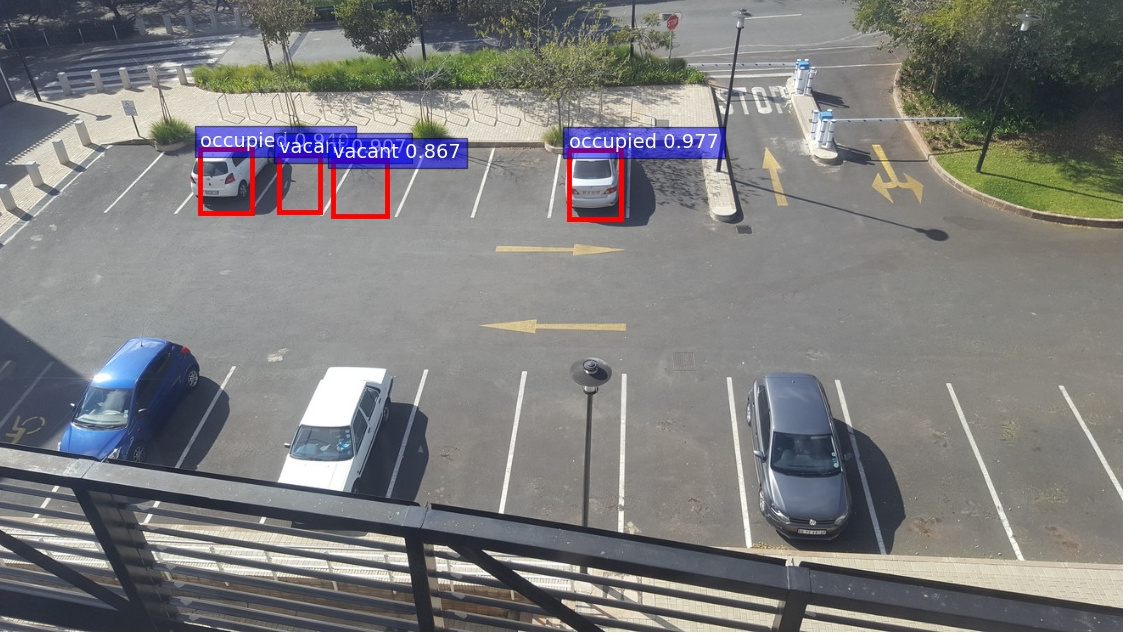
\includegraphics[width=0.7\linewidth]{Pictures/3}
	\caption{Sample Result of RCNN}
	\label{rcnn_example}
\end{figure}

\end{frame}

\begin{frame}
\frametitle{SVMs}
Have been broadly used previously. The hyper-parameters of the SVMs, C, $\gamma$, kernel will be computed using grid search. 
\end{frame}

\begin{frame}
\frametitle{Selection or Assignment of Parking Space: Conflict management}
\textbf{Automatic assignment}: 
\begin{itemize}
	\item Fill the bottom rows first,
	\item May not be followed as planned, which leads to method 2,
\end{itemize}

\textbf{Metered booking: }
\begin{itemize}
	\item Let the user book an available spot,
	\item Cancel booking after a period X of time,
	\item If same time booking happens: User1 and User3 book the spotA at the same time $t$, nodern DBMS are able to handle that case, otherwise, cancel both booking processes.
\end{itemize}
\end{frame}

\begin{frame}[allowframebreaks]
\frametitle{The Data: From A to Z} 
\textbf{Data Collection}
\begin{itemize}
	\item Mostly collected from the 4th, 3rd, Postgraduate Students parking next the Chamber of Mines , Wits
	\item With a GoPro Hero 4 camera,
\end{itemize}
\textbf{Data Preparation}
\begin{itemize}
	\item GoPro camera = Distortion $\implies$ distortion removal mainly,
	\item Reduction of the image size.
\end{itemize}
\textbf{Data Labeling}
\begin{itemize}
	\item \textbf{Detection}: Create ground-truth of all spots appearing in the collected pictures  in XML format,
	The input is the original image and the output a tuple $t$ = $\lbrace image.jpg,image.xml\rbrace$
	\item \textbf{Classification}: Generate patches of individual spots from all the pictures collected, regardless the state of the patch.
\end{itemize}
\framebreak
\textbf{Datasets}
\begin{itemize}
	\item \textbf{Training}: Generate 2 folders corresponding to the states of interest: Vacant and Occupied.
	\item \textbf{Testing}: PKLot dataset will be used, and some other scenarios of parking spaces different from the training ones.
\end{itemize}

\end{frame}

\begin{frame}[allowframebreaks]
\frametitle{Training \& Testing} 

\textbf{Detection}: 
\begin{itemize}
\item Caffe implementation of the Region-based CNN (RCNN) 
\item Different solvers type (Stochastic Gradient Descent Adaptive Gradient, Nesterov’s Accelerated Gradient ...) and learning rate, learning rate policy for better choice of accuracy,
\end{itemize}
\textbf{CNN Classification}:
\begin{itemize}
	\item Caffe or hdf5 (Keras) model for classifying the crop image of the parking spot,
	\item Feeding the CNN (no matter what model used) with the patches of parking lots collected from the dataset (vacant \& occupied folders).
\end{itemize}
\textbf{SVM Classification}: 
\begin{itemize}
	\item Using the winning feature extractors HOG, SURF, SIFT ...
	\item Using grid search to determine the optimal hyper-parameters of the proposed SVM model generated,
	\item Using $k$-fold cross-validation to efficiently train and test and avoid leaks of the training set to the testing set compared to using a static training-testing phase.
\end{itemize} 

\end{frame}

\begin{frame}[allowframebreaks]
\frametitle{How Will We Evaluate The Model?}

\textbf{Confusion Matrix}: Table or matrix to visually evaluate the performance of a model. This research project is a supervised learning binary classification problem. The resulting confusion matrix will produce four outcomes:
	\begin{itemize}
		\item \textbf{T}rue \textbf{N}egatives (\textbf{TN}): Actual negative outcomes that are predicted negatives,
		\item \textbf{T}rue \textbf{P}ositives (\textbf{TP}): Actual positive outcomes that are predicted positives,
		\item \textbf{F}alse \textbf{N}egatives (\textbf{FN}): Actual positive outcomes that are predicted negatives,
		\item \textbf{F}alse \textbf{P}ositives (\textbf{FP}): Actual negative outcomes that are predicted positives.
	\end{itemize}
	
	\begin{table}[!h]
		\centering
		\begin{tabular}{cc|c|c|c}
			\cline{3-4}
			& & \multicolumn{2}{ c| }{Predicted Classes} \\ \cline{3-4}
			& & Occupied & Vacant \\ \cline{1-4}
			\multicolumn{1}{ |c  }{\multirow{2}{*}{Actual Classes} } &
			\multicolumn{1}{ |c| }{Occupied} & \textbf{TN} & \textbf{FP} &     \\ \cline{2-4}
			\multicolumn{1}{ |c  }{}                        &
			\multicolumn{1}{ |c| }{Vacant} & \textbf{FN} & \textbf{TP} &     \\ \cline{1-4}
		\end{tabular}
		\caption*{Confusion Matrix: By convention, the true classes are on the left-hand side of the matrix and the predicted classes are on the top of the matrix.}
		\label{conmat}
	\end{table}

\begin{itemize}
	\item Accuracy = $\frac{\text{Total number of correct classication}}{\text{Total number of cases}}$ = $\frac{\textbf{TP + TN}}{\textbf{TP + TN + FN + FP}}$
	\item Recall = $\frac{\text{Number of True Positives}}{\text{Total number of actual positives}}$ = $\frac{\textbf{TP}}{\textbf{TP + FN}}$
	\item Precision= $\frac{\text{Number of True Positives}}{\text{Total number of predicted positives}}$ = $\frac{\textbf{TP}}{\textbf{TP + FP}}$
	\item \textbf{Receiver Operating Characteristic curve (ROC) curve} = \textbf{TPR} vs \textbf{FPR} = $\frac{\textbf{TP}}{\textbf{TP + FN}}$ (y-axis) vs $\frac{\textbf{FP}}{\textbf{FP + TN}}$ (x-axis): In that graph, the goal is to obtain a curve growing towards the upper right corner, reducing the number of false negatives and false positives as illustrated in Figure \ref{fig:roc}.
	
	\begin{figure}[!h]
		\centering
		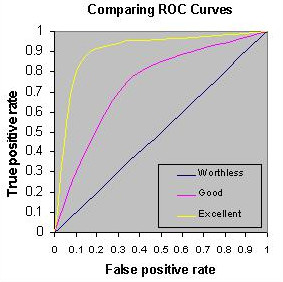
\includegraphics[width=0.6\linewidth]{Pictures/ROC}
		\caption{Three different cases of ROC curves, \citet{rocref}}
		\label{fig:roc}
	\end{figure}

	\item \textbf{Precision Recall Curve} = \textbf{Precision} (y-axis) vs \textbf{Recall} (x-axis): : In that graph, the goal is to obtain a curve growing towards the upper right corner, reducing the number of false positives as illustrated in Figure \ref{fig:precisionrecall}.

	
\begin{figure}[h!]
	\centering
	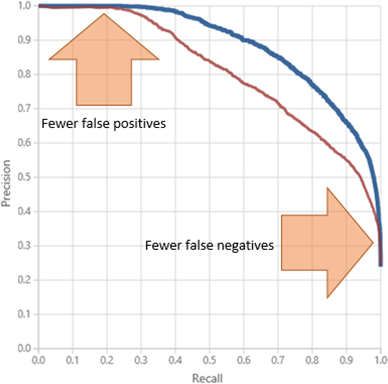
\includegraphics[width=0.5\linewidth]{Pictures/Precision_recall}
	\caption{Different cases of precision-recall curves, \citet{prref}}
	\label{fig:precisionrecall}
\end{figure}

\end{itemize}

\end{frame}

\begin{frame}[allowframebreaks]
\frametitle{Client Interface For Locating Vacant Parking Spaces}

\begin{figure}
	\centering
	\includegraphics[width=0.7\linewidth]{../../Project_Proposal/Pictures/Client_Server}
	\caption{Describes how the video frames containing the images the parking lot leave the camera to the computer that has the Automated Parking Space Detection system. After the images data have processed by the system, the result, which is a JSON file, is sent to the server. The server will then send the JSON file to the android phone when requested by the user.}
	\label{fig:clientserver}
\end{figure}


\end{frame}



\section{Research Plan}

\begin{frame}
\Huge Research Plan
\end{frame}

\begin{frame}
\frametitle{Research Phases and Time Plan}

\begin{table}[h!]
	\centering
	\begin{center}
		\begin{tabular}{ | l | l | l |}
			\hline
			\textbf{Phase} & \textbf{Duration} & \textbf{\# of weeks} \\ \hline
			Data collection & June 2017- August 2017 & 12 weeks \\ \hline
			Data Preparation & August 2017- October 2017 & 12 weeks \\ \hline
			Training \& Testing & October 2017- February 2018 & 16 weeks \\ \hline
			Deployment & February 2018- April 2018 & 12 weeks \\ \hline
			Analysis & March 2018- June 2018 & 16 weeks \\ \hline			
			Write-up & July 2018- September 2018 & 12 weeks \\ \hline
			
		\end{tabular}
	\end{center}
	\caption{Research Phases and Time Plan}
	\label{timeplan}
\end{table}

\end{frame}

\begin{frame}
\frametitle{Potential Issues and Risk Management}
\begin{itemize}
	\item \textbf{Data Collection Issues}:\\
	The data will be collected by the researcher if there is no, or not usable footage available,
	\item \textbf{Delays on Defined Time Plan}:\\
	The design of the different components may take longer to produce, that will generate a delay on the delivery time,
\end{itemize}
\end{frame}
%----------------------------------------
\section{What's next}

\begin{frame}
\frametitle{Path to follow}
\begin{block}{Guidelines}
Our main objectives will be to:
\begin{itemize}
\item Compare the performance of the mainly used classifiers based on the literature review: CNN and SVM,
\item Collect data for the new experiments to do based on the classifier we will choose,
\item Design and implement an algorithm that will automatically withdraw the parking bays to feed them to the classifier (Hough transform for example) given the whole parking lot
\item Perform a qualitative analysis of the usage of the parking as a whole to predict the availability of the bays.

\end{itemize}

\end{block}
\end{frame}

%-----------------------------------------------

\begin{frame}
\Huge{\centerline{End}}
\end{frame}

%----------------------------------------------------------------------------------------

%------------------------------------------------
\section{References}
%------------------------------------------------
\begin{frame}[allowframebreaks]{References}%in case more than 1 slide needed
\footnotesize{
\bibliographystyle{ieeetr}
\bibliography{reference.bib}}
\end{frame}
\end{document}

\end{document}